% §5 Empirical evidence (dimension-wise characterization)

We present \textbf{empirical evidence} for the routing question on ARC-Challenge test ($n{=}1{,}172$).
The analytic question throughout is dimensional: \textbf{which latent routing dimension predicts routing opportunity?}---not which statistic ranks highest in isolation.

\subsection{Overview}
\label{sec:char:conceptual}

Figure~\ref{fig:conceptual} summarizes the paper: routing problem $\rightarrow$ operationalized dimensions $\rightarrow$ appropriate model selection.

\begin{figure}[t]
  \centering
  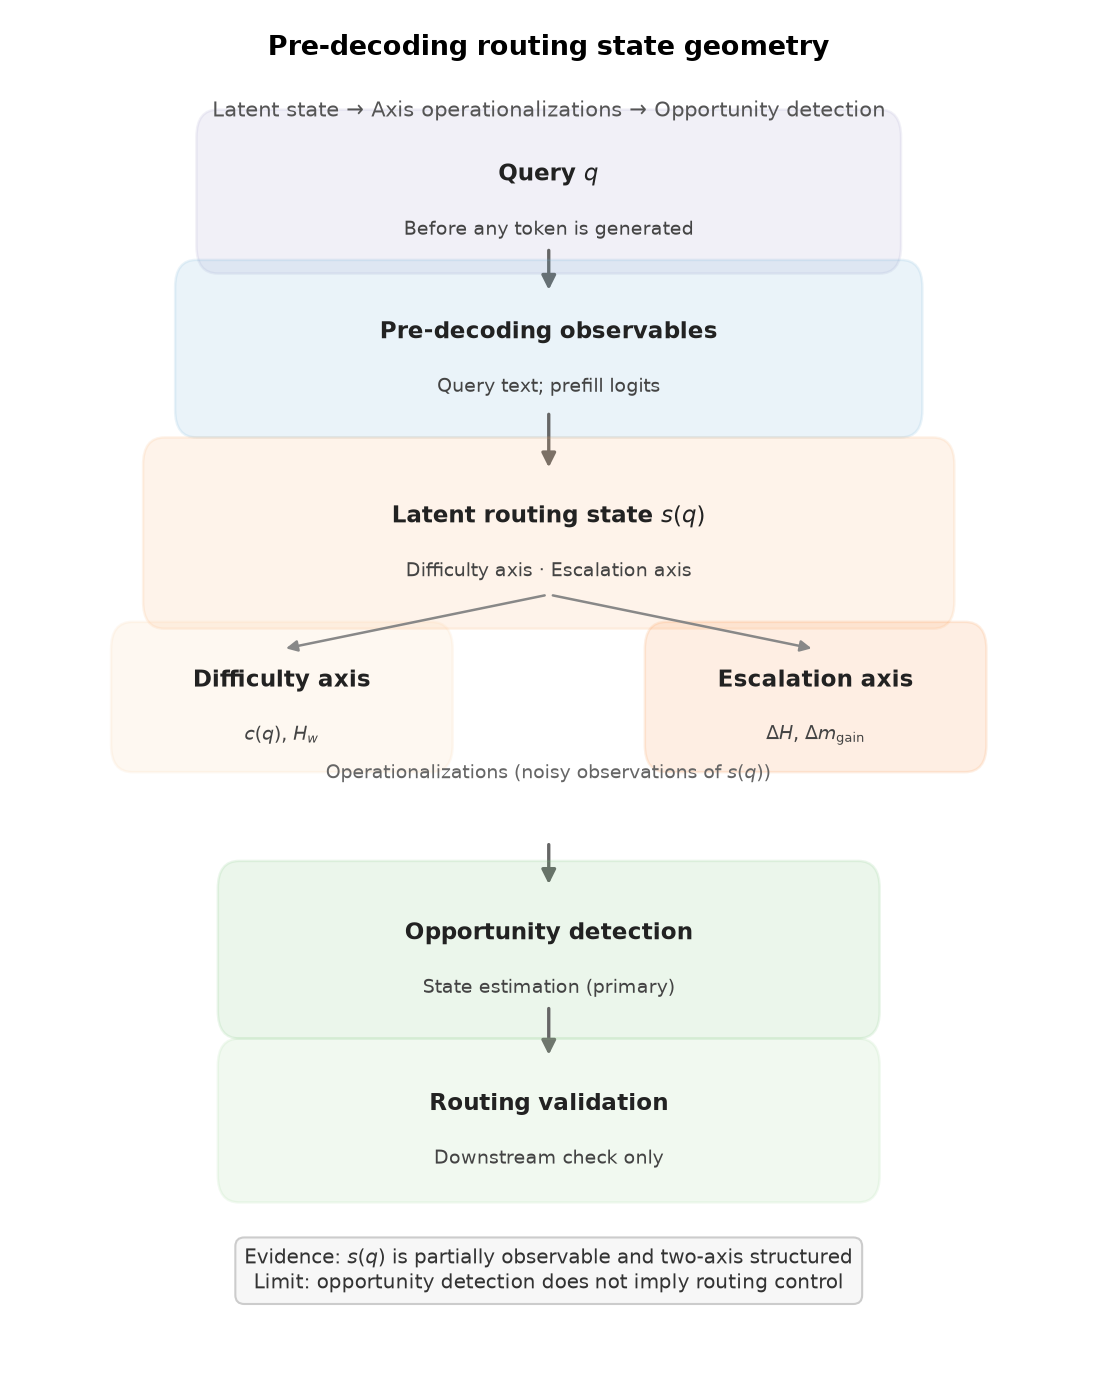
\includegraphics[width=\linewidth]{figures/F0_conceptual_model.png}
  \caption{Unsupervised pre-inference routing via \textbf{latent routing dimensions}. Each dimension is operationalized by a prefill statistic; the scientific unit is the dimension, not the statistic.}
  \label{fig:conceptual}
\end{figure}

\subsection{Finding 1: Latent dimensions predict routing opportunity}
\label{sec:char:finding1}

\paragraph{Oracle landscape.}
Table~\ref{tab:buckets} summarizes offline oracle buckets (\S\ref{sec:setup:oracle}).
Routing opportunity occurs on 43.3\% of test queries---the label each dimension is tested against.

\begin{table}[t]
  \centering
  \small
  \begin{tabular}{lrr}
    \toprule
    \textbf{Bucket} & \textbf{Count} & \textbf{Rate} \\
    \midrule
    Easy & 304 & 25.9\% \\
    Opportunity & 507 & 43.3\% \\
    Weak-only & 61 & 5.2\% \\
    Too-hard & 300 & 25.6\% \\
    \midrule
    \textbf{Total} & \textbf{1{,}172} & \textbf{100\%} \\
    \bottomrule
  \end{tabular}
  \caption{Oracle bucket distribution on ARC test.}
  \label{tab:buckets}
\end{table}

\paragraph{Dimension-wise predictiveness (Studies I--II).}
Table~\ref{tab:study2} reports, for each operationalized dimension, association with $y^{\text{opp}}$.
\textbf{Escalation potential} ($\Delta m_{\mathrm{gain}}$) and \textbf{model disagreement} ($\Delta H$) are the strongest predictors (AUROC ${\sim}0.60$--$0.61$); \textbf{task difficulty} is weaker (AUROC $0.541$).
\textbf{Multiple dimensions carry predictive content}, but none approaches perfect opportunity detection.

% T2: which latent routing dimension predicts opportunity? (ARC TEST)
\begin{table}[t]
  \centering
  \small
  \begin{tabular}{llccc}
    \toprule
    \textbf{Latent routing dimension} & \textbf{Operationalization} & $\rho_s$ [95\% CI] & AUROC [95\% CI] & AUPRC \\
    \midrule
    Task difficulty & $c(q)$ & $+0.071$ [$+0.015$, $+0.128$] & $0.541$ [$0.509$, $0.574$] & $0.474$ \\
    Model uncertainty & $H_w$ & $+0.138$ [$+0.082$, $+0.193$] & $0.581$ [$0.547$, $0.613$] & $0.500$ \\
    Model disagreement & $\Delta H$ & $+0.174$ [$+0.118$, $+0.232$] & $0.602$ [$0.569$, $0.635$] & $0.559$ \\
    Escalation potential & $\Delta m_{\mathrm{gain}}$ & $+0.179$ [$+0.123$, $+0.239$] & $0.605$ [$0.572$, $0.637$] & $0.547$ \\
  \end{tabular}
  \caption{Which \textbf{latent routing dimension} predicts routing opportunity? Predictive association of each operationalized dimension with $y^{\text{opp}}$ on ARC test ($n{=}1{,}172$). AUROC summarizes detectability; the scientific question is dimensional, not a feature leaderboard.}
  \label{tab:study2}
\end{table}


\begin{figure}[t]
  \centering
  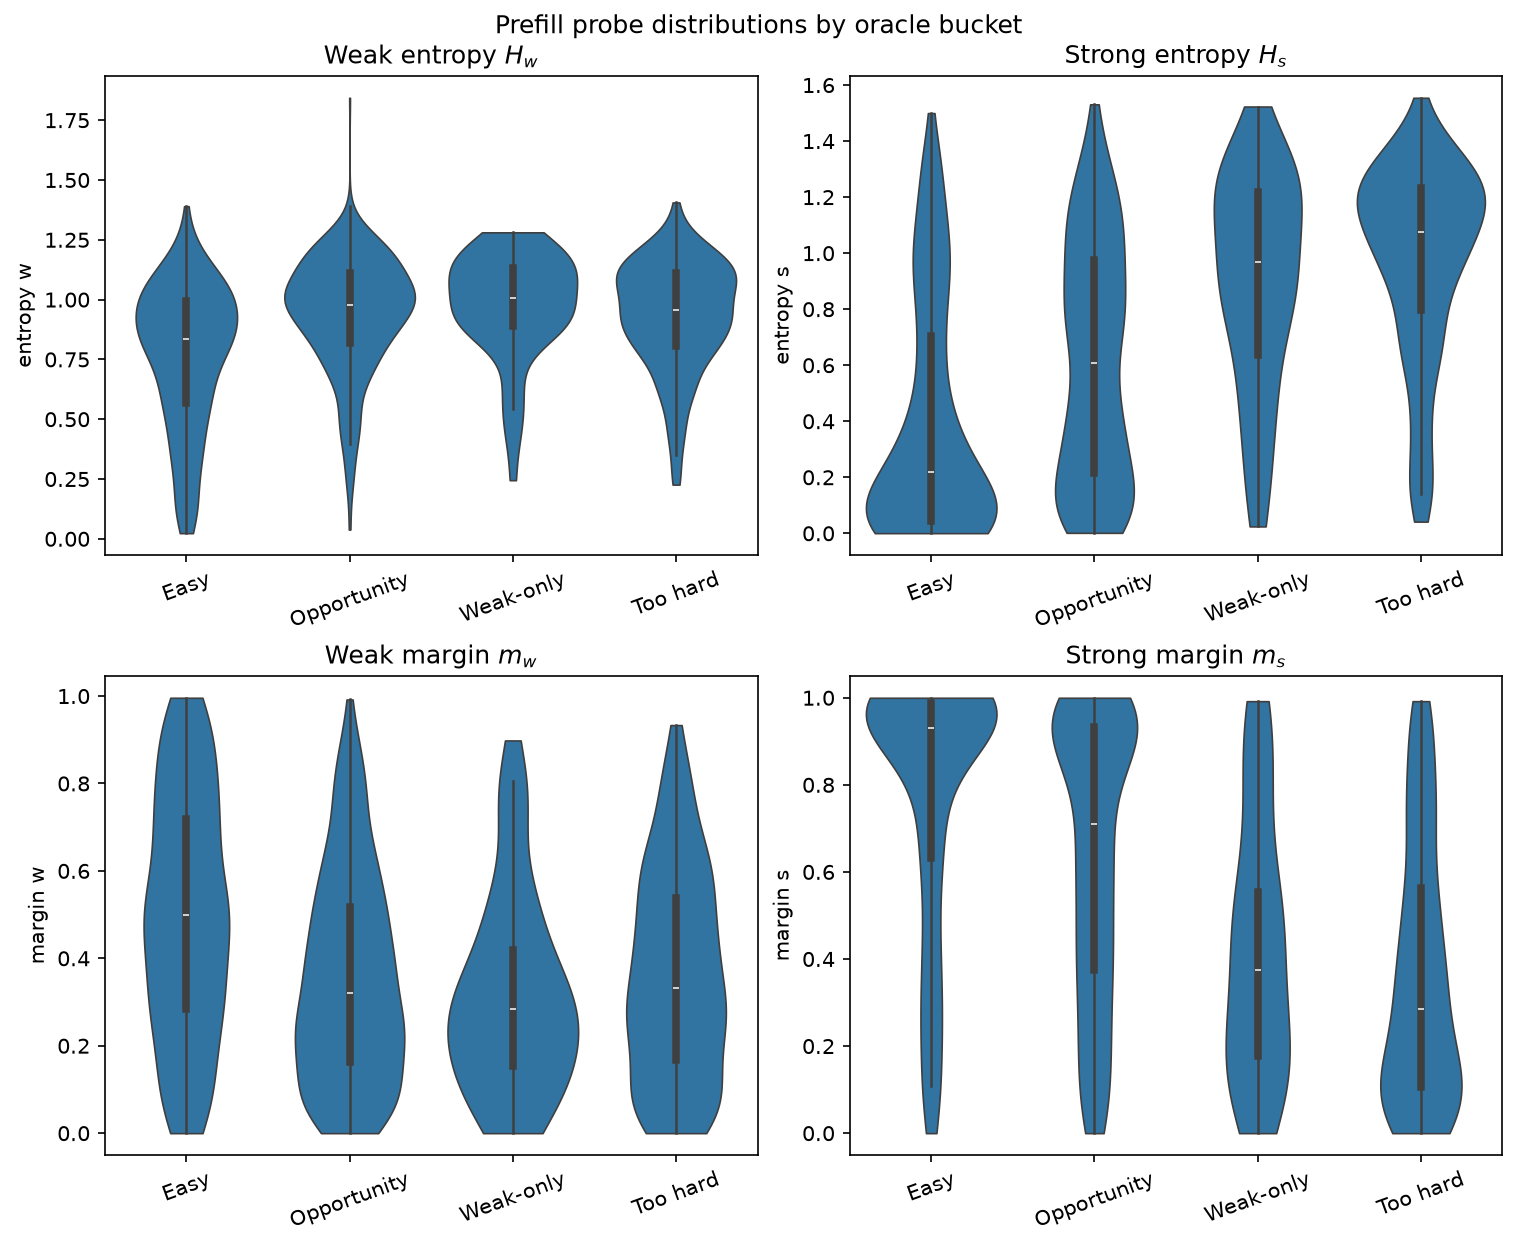
\includegraphics[width=\linewidth]{figures/F1_bucket_distributions.png}
  \caption{Operationalized dimensions by oracle bucket on ARC test.}
  \label{fig:signal-dist}
\end{figure}

\subsection{Finding 2: Dimensions encode different aspects of routing need}
\label{sec:char:finding2}

\paragraph{Cross-dimension structure.}
Dimensions are not interchangeable predictors of the same latent quantity.
Figure~\ref{fig:semantics} contrasts \textbf{model uncertainty} ($H_w$) with \textbf{escalation potential} ($\Delta m_{\mathrm{gain}}$)---both from prefill logits but indexing different routing need.

\begin{figure}[t]
  \centering
  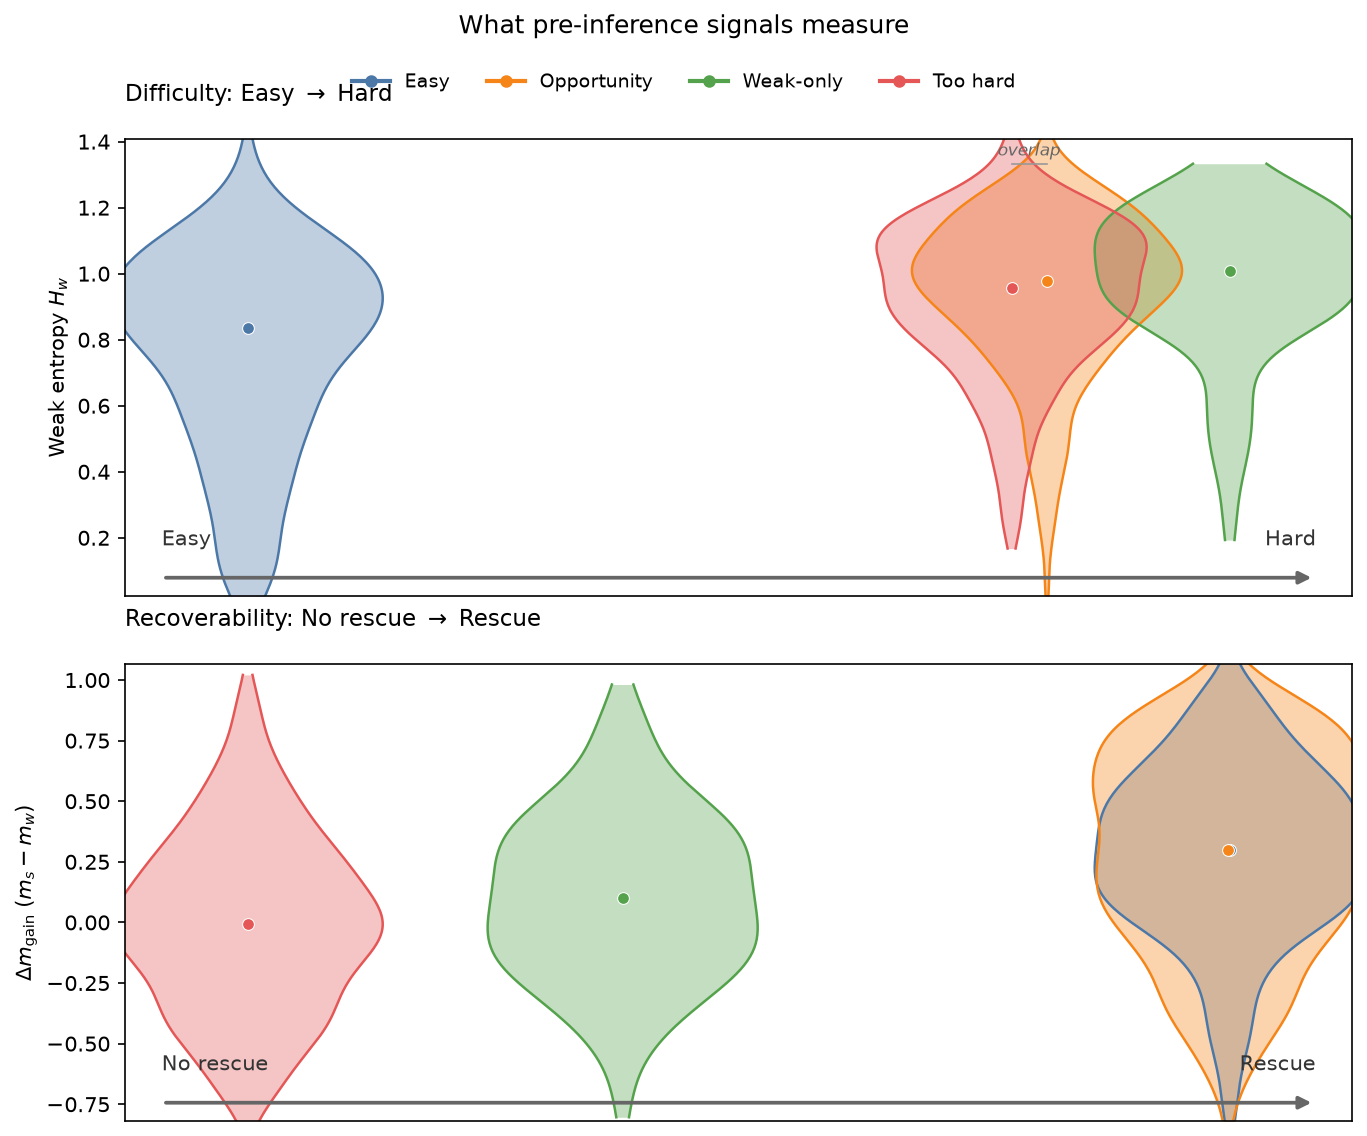
\includegraphics[width=\linewidth]{figures/F2_signal_semantics.png}
  \caption{Model uncertainty vs.\ escalation potential, by oracle bucket.}
  \label{fig:semantics}
\end{figure}

\paragraph{Opportunity vs.\ too-hard.}
Comparing opportunity ($n{=}507$) and too-hard ($n{=}300$):
model uncertainty ($H_w$): $d{\approx}0.03$; escalation potential ($\Delta m_{\mathrm{gain}}$): $d{\approx}0.72$; model disagreement ($\Delta H$): $d{\approx}0.82$.
\textbf{Difficulty-side dimensions} (task difficulty, model uncertainty) do not separate routable from irrecoverable hard queries; \textbf{escalation-side dimensions} (model disagreement, escalation potential) do.

\paragraph{Recovery matrix.}
Figure~\ref{fig:recovery} crosses model uncertainty and escalation potential (median splits).
Highest opportunity rate (57.2\%; $n{=}353$): weak-uncertain queries where the strong model rescues.

\begin{figure}[t]
  \centering
  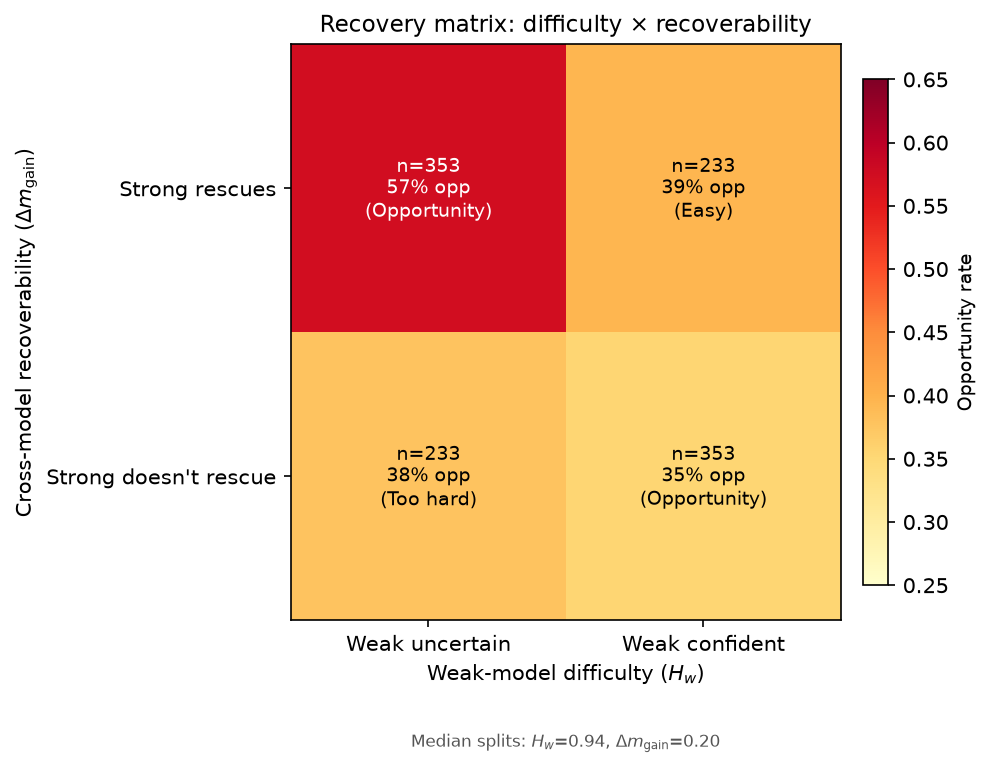
\includegraphics[width=0.92\linewidth]{figures/F6_recovery_matrix.png}
  \caption{Opportunity rate by model uncertainty ($H_w$) and escalation potential ($\Delta m_{\mathrm{gain}}$).}
  \label{fig:recovery}
\end{figure}

\subsection{Complementary predictive content (Study III)}
\label{sec:char:study3}

Adding \textbf{model uncertainty} to \textbf{task difficulty} yields $\Delta$AUROC $= +0.049$ (DeLong $p{=}0.008$): the two dimensions capture partially non-redundant predictive content.
An alternate operationalization of uncertainty ($m_w$) does not improve the joint model on ARC.
Figure~\ref{fig:decomposition} and Table~\ref{tab:complementarity} summarize the dimensional ladder.

% T3: Study III — complementarity ladder (fill after complementarity JSON)
\begin{table}[t]
  \centering
  \small
  \begin{tabular}{lcc}
    \toprule
    \textbf{Model} & \textbf{Features} & AUROC [95\% CI] \\
    \midrule
    Complexity only & $c(q)$ & TBD \\
    Entropy only & $H_w$ & TBD \\
    Margin only & $m_w$ & TBD \\
    $c + H$ & $c, H_w$ & TBD \\
    $c + m$ & $c, m_w$ & TBD \\
    \textbf{Joint (primary)} & $c, H_w, m_w$ & \textbf{TBD} \\
    \midrule
    $\Delta$AUROC ($c \rightarrow c{+}H{+}m$) & --- & \textbf{TBD} \\
    DeLong $p$ & --- & TBD \\
    \bottomrule
  \end{tabular}
  \caption{Study III (RH3): complementary predictive information on ARC test. Primary endpoint: $\Delta$AUROC from $c(q)$ to $c{+}H_w{+}m_w$.}
  \label{tab:complementarity}
\end{table}


\begin{figure}[t]
  \centering
  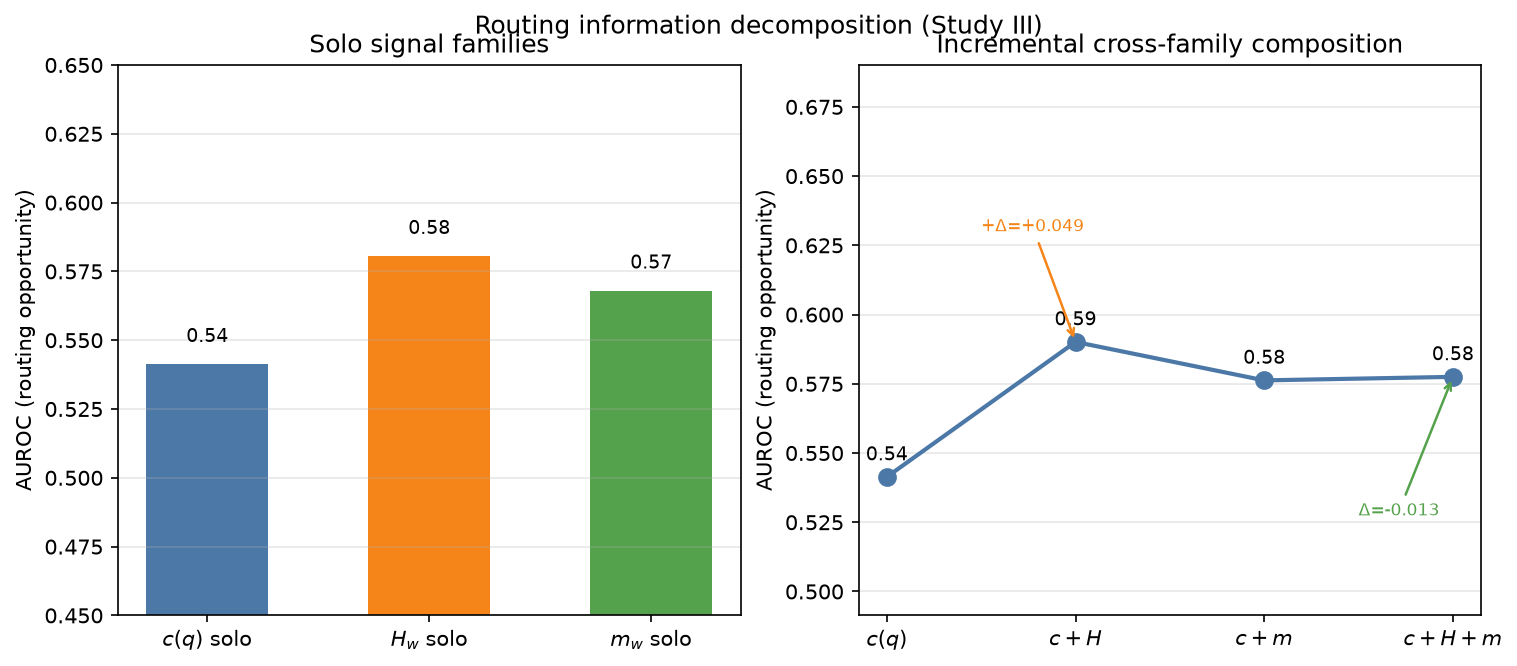
\includegraphics[width=\linewidth]{figures/F3_information_decomposition.png}
  \caption{Complementarity across operationalized dimensions (CALIB-fit, TEST-eval).}
  \label{fig:decomposition}
\end{figure}

\subsection{Probe cost}
\label{sec:char:cost}

Table~\ref{tab:probe-cost} compares prefill-probe cost to post-generation routing \citep{guha2024smoothie,kotte2026ucci,hu2024routerbench}.

\begin{table}[t]
  \centering
  \small
  \begin{tabular}{ll}
    \toprule
    \textbf{Strategy} & \textbf{Relative cost} ($m{=}2$) \\
    \midrule
    Always weak & 1 generation \\
    Always strong & 3 generations \\
    Prefill probes & $\ll 1$ generation \\
    Post-generation routing & 2 generations \\
    \bottomrule
  \end{tabular}
  \caption{Prefill probes vs.\ full generation cost.}
  \label{tab:probe-cost}
\end{figure}
